\documentclass[a4paper,12pt]{article}
\usepackage{blindtext}
\usepackage[utf8]{inputenc}
\usepackage{graphicx}

\begin{document}
\begin{titlepage}
\center

\textsc{\LARGE Project: Unit-Assess}\\[1.5cm]
\textsc{\Large Client: Mr Schalk Lotz, Magna BC}\\[0.5cm]
\textsc{\large Team: Quadcore Productions}\\[0.5cm]

\begin{minipage}{0.4\textwidth}
\begin{flushleft} \large
\emph{Author(s):}\\
Mpho \textsc{Baloyi}\\
Hlengekile \textsc{Jita}\\
Mayimela \textsc{Moses}\\
Mbhele \textsc{Themba}\\
\end{flushleft}
\end{minipage}
~
\begin{minipage}{0.4\textwidth}
\begin{flushright} \large
\emph{Student number(s):} \\
14133670\\ % Student number
14077893\\
14019702\\
14007950\\
\end{flushright}
\end{minipage}\\

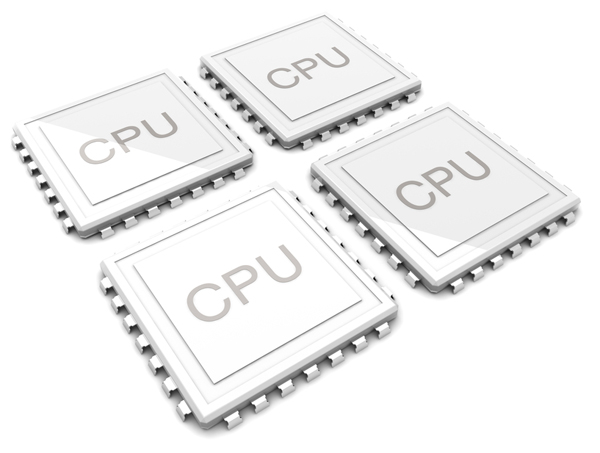
\includegraphics[width=\textwidth]{2012-quad-core-phones}

{\large University of Pretoria, Department of Computer Science}\\

{\large 02 May 2016}\\[3cm]

\vfil

\end{titlepage}

\newpage

\section{The Team}
\subsection{Mpho Baloyi}
\subsubsection{Interests}
\begin{itemize}
\item Keeping abreast with new technologies
\item Learning and using new technologies to solve problems
\item Reading up and doing research on new and old concepts in computer science
\item Solving riddles and puzzles
\item Helping people through ICT
\end{itemize}
\subsubsection{Technical Skills}
\begin{itemize}
\item Solid programming skills in java,c++ and python
\item Fair amount of knowlegde in assembly programming
\item Web development with HTML,JAVASCRIPT,JQUERY,CSS,PHP,AJAX,ANGULARJS
\item Interaction Design
\item Database design with MySQL
\item Understanding of process development
\item Unit testing,mocking and dependency Injection
\end{itemize}
\subsubsection{Non-Technical Strengths}
\begin{itemize}
\item Exellent Communication skills
\item Patient
\item Creative approach to problem solving
\item Pay attention to detail
\item Excellent planning skills
\item Ability to grasp concepts quickly
\item Willness to learn new things
\item Ability to interpret and follow technical plans
\item Ability to collaborate and work efficiently with other people
\item Ability to work under pressure
\end{itemize}
\subsubsection{Relevant Past Experiences}
\subsubsection{Reasons for wanting to do the project}
I want to do this project because it provides me with the opportunity to work with different kinds of technologies and devices and to learn new ways of collecting data.
\subsection{Hlengekile Jita}
%\includegraphics[width=\textwidth]{}
\subsubsection{Interests}
\subsubsection{Technical Skills}
\subsubsection{Non-Technical Strengths}
\subsubsection{Relevant Past Experiences}
\subsubsection{Reasons for wanting to do the project}
\subsection{Moses Mayimela}
%\includegraphics[width=\textwidth]{}
\subsubsection{Interests}
\subsubsection{Technical Skills}
\subsubsection{Non-Technical Strengths}
\subsubsection{Relevant Past Experiences}
\subsubsection{Reasons for wanting to do the project}
\subsection{Themba Mbhele}
%\includegraphics[width=\textwidth]{}
\subsubsection{Interests}
\subsubsection{Technical Skills}
\subsubsection{Non-Technical Strengths}
\subsubsection{Relevant Past Experiences}
\subsubsection{Reasons for wanting to do the project}
\section{Project Execution}
\subsection{Development Methodology}
\subsection{Communication With Client}
To keep the clients informed we are going to use the following means of communication
\subsubsection{email}
\begin{itemize}
\item To inform the client of our progress
\item To address any issues or concerns that they client may have
\item To acquire information from the client
\item To require any resources that the client has to offer for their project,..
\end{itemize}
\subsubsection{Regular Meetings}
These will take place depending on the clients availability and willingness.
We may discuss the progress of the project,to address any concerns,etc.
\subsubsection{GIT}
Access to our git repository will be provided to the client,so the client can be able to monitor
our progress and have access to the project material.
We are also open to any means of communication that the client may prefer or suggest.
\subsection{Technical Challenges}

\end{document}
